% ---------------------------------------------------------------------------
% Author guideline and sample document for EG publication using LaTeX2e input
% D.Fellner, v1.13, Nov 13, 2007


\documentclass{egpubl}

% --- for  Annual CONFERENCE
% \ConferenceSubmission % uncomment for Conference submission
% \ConferencePaper      % uncomment for (final) Conference Paper
% \STAR                 % uncomment for STAR contribution
% \Tutorial             % uncomment for Tutorial contribution
% \ShortPresentation    % uncomment for (final) Short Conference Presentation
%
% --- for  CGF Journal
% \JournalSubmission    % uncomment for submission to Computer Graphics Forum
% \JournalPaper         % uncomment for final version of Journal Paper
%
% --- for  CGF Journal: special issue
% \SpecialIssueSubmission    % uncomment for submission to Computer Graphics Forum, special issue
% \SpecialIssuePaper         % uncomment for final version of Journal Paper, special issue
%
% --- for  EG Workshop Proceedings
% \WsSubmission    % uncomment for submission to EG Workshop
% \WsPaper         % uncomment for final version of EG Workshop contribution
%

\electronicVersion % can be used both for the printed and electronic version

% !! *please* don't change anything above
% !! unless you REALLY know what you are doing
% ------------------------------------------------------------------------

% for including postscript figures
% mind: package option 'draft' will replace PS figure by a filname within a frame
\ifpdf \usepackage[pdftex]{graphicx} \pdfcompresslevel=9
\else \usepackage[dvips]{graphicx} \fi

\PrintedOrElectronic

% prepare for electronic version of your document
\usepackage{t1enc,dfadobe}
\usepackage[utf8]{inputenc}
\usepackage{egweblnk}
\usepackage{cite}
\usepackage{amssymb}
\usepackage{amsmath}
\usepackage[T1]{fontenc}

%\usepackage[
%    top    = 1.32in,
%    bottom = 1.32in,
%    left   = 0.96in,
%    right  = 0.96in]{geometry}

%\usepackage[spanish]{babel}

%\usepackage[spanish,activeacute]{babel}
%\usepackage[spanish]{translator}

\newcommand{\bigO}{\mathcal{O}}



% For backwards compatibility to old LaTeX type font selection.
% Uncomment if your document adheres to LaTeX2e recommendations.
\let\rm=\rmfamily    \let\sf=\sffamily    \let\tt=\ttfamily
\let\it=\itshape     \let\sl=\slshape     \let\sc=\scshape
\let\bf=\bfseries

% end of prologue

% ---------------------------------------------------------------------
% EG author guidelines plus sample file for EG publication using LaTeX2e input
% D.Fellner, v1.16, Jan 21, 2009


\title[EG \LaTeX\ Author Guidelines]%
      {A$^*$mbush: una Variación de A$^*$ para Generar Emboscadas y Diversidad de Caminos}

% for anonymous conference submission please enter your SUBMISSION ID
% instead of the author's name (and leave the affiliation blank) !!
\author[K. Fernández, G. González,  C. Chang]
       {K. Fernández, G. González,  C. Chang
%        S. Spencer$^2$\thanks{Chairman Siggraph Publications Board}
        \\
% For Computer Graphics Forum: Please use the abbreviation of your first name.
         Grupo de Inteligencia Artificial, Departamento de Computación y Tecnología de la Información, Universidad Simón Bolívar, Venezuela\\
      }

% ------------------------------------------------------------------------

% if the Editors-in-Chief have given you the data, you may uncomment
% the following five lines and insert it here
%
% \volume{27}   % the volume in which the issue will be published;
% \issue{1}     % the issue number of the publication
% \pStartPage{1}      % set starting page


%-------------------------------------------------------------------------
\begin{document}
\noEGpagenumber

\maketitle

\begin{abstract}
En el área de Inteligencia Artificial para videojuegos, A* es
un algoritmo comúnmente propuesto para generar caminos que 
utilizarán los agentes autónomos. Aunque A* garantiza
optimalidad, tiende a producir conductas similares en elementos que
estén cercanos entre ellos y no asegura un ataque por diversos flancos
cuando los agentes están distribuidos de manera esparcida. Para generar
conductas de emboscada y diversidad de caminos, se propone una modificación 
del algoritmo llamada A*mbush, que considera para el costo de los nodos (o arcos), 
la cantidad de agentes que tienen calculado ese punto dentro de su camino hacia
la meta.
\\
\textbf{Palabras claves:} A*, estrategias grupales, búsqueda de caminos.
\\
\\
\textnormal{\textbf{ABSTRACT}}
\\
\\
In the area of Artificial Intelligence for Videogames, A* is a commonly proposed 
algorithm for path-finding. Even though this algorithm guaranties optimality, it 
tends to bring forth similar behaviours in agents that are close to each other. On the
other hand, when the agents are sparsely distributed, the algorithm doesn't secure
an attack that comes from different places. Having the generation of ambush
behaviours and diversity of paths as the goal, A*mbush is proposed. It is a 
modification of A* that considers the amount of agents that have a specific
node (or edge) in their calculated path, when it's computing the cost function of that 
point in the graph.


%
\begin{keywords}
A*, estrategias grupales, búsqueda de caminos.
\end{keywords}

\end{abstract}





%-------------------------------------------------------------------------
\section{Introducción}

En el área de Inteligencia Artificial para Videojuegos, generar
agentes con conductas que luzcan inteligentes para el
usuario, es un reto constante \cite{MF09}. Entre estos comportamientos,
el usuario espera apreciar agentes que desarrollen movimientos
tácticos y estratégicos grupales, los cuales suelen ser sumamente
complejos de implementar. Esto muchas veces genera como resultado
acciones prestablecidas que el usuario puede fácilmente identificar después
de varias ejecuciones del juego.

Un problema muy tratado es la búsqueda de caminos a un punto común,
por parte de grupos de agentes dentro de un juego \cite{MF09}. Este punto suele
venir dado por un lugar en el mapa de juego, potencialmente la
posición del oponente.
El esquema regularmente utilizado es generar caminos de costo mínimo
\cite{HNR72} \cite{RN93}
hacia este punto, sobre el grafo inducido por el mapa del juego. Es
muy probable, que estos caminos confluyan, evitando la diversidad de
rutas y exploración del mapa.

Al efectuar una persecución al oponente, la utilización de caminos
óptimos como estrategia deja muchos espacios de escapatoria libres,
por lo que es de especial interés generar mecanismos de diversificación de
rutas que generen situaciones de emboscada.

La técnica expuesta próximamente es adaptable a muchos contextos en
los que, si bien no es necesaria una situación de emboscada, es
importante generar diversidad de caminos con el fin de no sobresaturar
ciertos sectores del grafo subyacente. Ejemplo de estos son controladores
de tráfico, enrutamiento de paquetes físicos o digitales \cite{TMSV03},
robótica, entre otros.

%-------------------------------------------------------------------------

\section{Definición Formal del Problema}

Sea $G = (V,E)$ un grafo (dirigido o no), donde
$V$ es el conjunto de nodos y $E$
el conjunto de arcos.

Sea $A$ un conjunto de agentes
interesados en alcanzar un punto $t \in V$. Se tiene
que cada agente $i \in A$, se encuentra en algún nodo del grafo
denominado $pos(i)$. Además, se define para $i$ la función
de costos de su desplazamiento por el grafo
$\lambda_i : E \longrightarrow \mathbb{R}^{\geq 0}$.

Se considera, sin pérdida de generalidad, que $V$ y $E$ son comunes para
todos los agentes, con el fin de no generar inconsistencias en la
información compartida entre estos. Sin embargo, cada agente puede tener
función de costos distintas, adaptadas a sus restricciones.

Sea $path(i)$ con $i \in A$, el camino que está siguiendo el agente
$i$ hasta el nodo $t$.

Se define el grado de emboscada del nodo $t$ como:

$\Phi(t) = \dfrac{|\{ i : path(j) = <pos(j),\ \ldots,\ i,\ t>, j \in A\}|}
	  {\min(|\{ <i,t> : <i,t> \in E \} |,|A|) }$

Es decir, la proporción de nodos adyacentes al nodo $t$,
desde los cuales algún agente está alcanzándolo con
respecto al máximo número de nodos adyacentes a $t$ mediante
los cuales, los agentes en $A$ podrían alcanzarlo. Por lo tanto,
$0 \leq \Phi(t) \leq 1$.

El objetivo de la variación propuesta es maximizar el valor
de $\Phi(t)$, dando prioridad a la diversidad de los caminos
considerados por el conjunto de agentes sobre su optimalidad.

\begin{figure}[htb]
	\begin{center}
		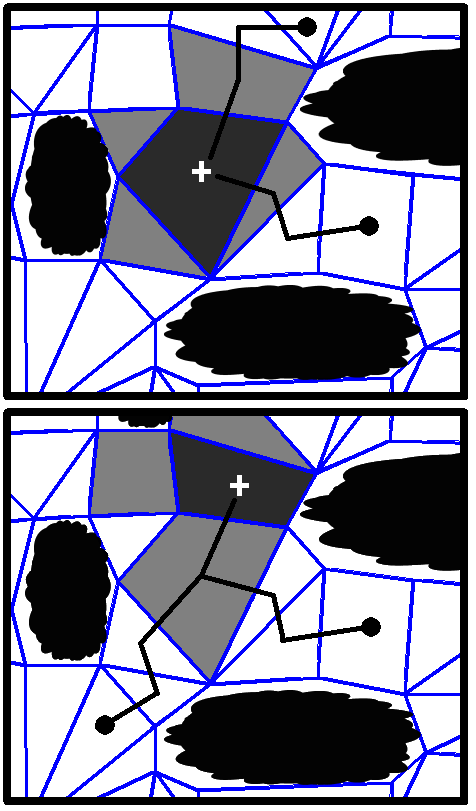
\includegraphics[scale=0.4]{ambush_rate.png}
	\end{center}
	\caption{\label{fig:phi}
	     Ejemplos de emboscadas con valores de $\Phi(t)$ 
	     1 y 0.5 respectivamente}
\end{figure}

Véase por ejemplo la figura \ref{fig:phi}, en ella se puede
observar en la imagen superior dos agentes situados en los
puntos negros. El objetivo a alcanzar por ambos agentes es
la cruz blanca situada en el polígono de color gris oscuro.
Los nodos ad\-ya\-cen\-tes al polígono objetivo se encuentran
demarcados con color gris claro.
Nótese que el número de polígonos adyacentes al destino es de
cuatro. De estos cuatro polígonos, sólo dos están siendo
considerados en los caminos de los agentes. Por lo tanto, el
valor $\Phi(t) = \dfrac{2}{min(4,2)} = 1$. Podría con\-si\-de\-rar\-se
que este tipo de emboscada no es óptimo dado que aún
quedan dos polígonos libres de escapatoria. Sin embargo,
es el mayor grado de emboscada posible dado que existen
sólo dos agentes.

En el segundo caso de la misma figura, puede a\-pre\-ciar\-se
una instancia en la cual de los tres posibles polígonos adyacentes
existe sólo uno siendo considerado en algún camino. Para este
caso, la métrica daría como resultado
$\Phi(t) = \dfrac{1}{min(3,2)} = 0.5$.

La importancia de considerar el mínimo entre el número de
nodos adyacentes y el número de agentes es no penalizar casos
como el primero, donde los caminos responden co\-rrec\-ta\-men\-te
al problema planteado.

\section{A*}

El algoritmo de A* \cite{HNR72} \cite{RN93} \cite{MF09}
 es una variación del algoritmo de Dijkstra \cite{CLRS09}
para cómputos de caminos de costo mínimo.

Consiste en un algoritmo de búsqueda informada \cite{RN93},
basado en los siguientes elementos:

\begin{itemize}
\item $g$: Es el costo acumulado desde el nodo inicial a un nodo actual $v$.
\item $\hat{h}$: Estimado del costo desde el nodo actual $v$ a la meta.
\item $\hat{f} = g + \hat{h}$: Estimado del costo desde el nodo inicial a la meta, pasando por $v$.
\end{itemize}

Para garantizar optimalidad, la heuristica $\hat{h}$ debe
ser admisible \cite{HNR72}, es decir, no debe estimar
costos mayores al óptimo del grafo.

El algoritmo actúa de forma voraz, expandiendo el 
si\-guien\-te nodo no explorado con menor costo estimado $\hat{f}$.
Este proceso continúa hasta llegar a la meta. 

En la figura \ref{fig:astar} puede apreciar un pseudocódigo del
algoritmo de $A^*$.

\begin{figure}[htb]
\begin{verbatim}
A_star(i, t):
    Para cada v en V:
        v.costo = inf
    pos(i).costo = 0

    nodo ini
    ini.v = pos(i)
    ini.f = 0
    ini.g = 0
    ini.h = h(v,t)
    ini.padre = null
    
    Mientras !vacia(q):
        nodo n = menor(q)
        extraer_menor(q)
        
        Si n.v = t:
            retornar reconstruir_camino(n)
        
        Si n.g > n.v.costo:
            continuar
        
        Para cada w sucesor de n.v:
            nodo s
            s.v = w
            s.h = h(w,t)
            s.g = n.g + lambda_i(<n.v, w>)
            s.f = s.g + s.h
            s.padre = v
            
            Si s.g < w.costo:
                agregar(q,s)
        Fin para
    Fin Mientras
\end{verbatim}
\caption{\label{fig:astar}
     Pseudocódigo del Algoritmo A* del agente $i$ con destino $t$.}
\end{figure}

% fin de la nueva def y luego viene lo del orden del algoritmo

En este caso, la complejidad asintótica en tiempo
del algoritmo de A* es de $\bigO(|V|log(|V|) + |V|*h + |E|)$,
con $h$ el costo de cómputo de la función $\hat{h}$,
suponiendo que se cuenta con una implementación eficiente de
cola de prioridades tal como un Fibonacci heap \cite{CLRS09} (estructura
de montículo que permite acceder al mínimo elemento del montículo
y agregar un elemento en tiempo constante; además de
e\-li\-mi\-nar uno en tiempo logarítmico amortizado) y que estamos
computando el costo heurístico de cada nodo una sola vez.

\section{A*mbush}

La variación propuesta al algoritmo $A^*$ para solucionar
el problema de generación de emboscadas A*mbush (por la
traducción al inglés de emboscada, ambush) consiste en
una modificación de la función $g$, que favorezca la
diversidad de caminos, a la cual denominaremos $g'$.

\subsection{Enfoque de Costos Agregados en Nodos}

Sea $\Psi(v,i) = 1+(\# j : j \in A \wedge v \in path(j))$,
el número de agentes distintos al agente $i$, que contienen al
nodo $v$ en sus caminos hasta $t$. Se considera que si un agente
no está buscando en dicho momento alcanzar el nodo $t$, o si
aún no ha realizado la búsqueda del camino, este es vacío, por
lo que no se consideran en el cómputo de $\Psi(v,i)$; dado
que $i$ no ha computado ya su camino hasta $t$, se considera
nulo su camino.

Para el nodo inicial, se considera $g'(pos(i),i) = 0$.
Sea $<v,w>$ el siguiente arco a considerar en la expansión del
nodo $v$ en una iteración cualquiera del algoritmo, se considera
$g'(w, i) = g'(v,i) + \lambda_i(<v,w>) \cdot \Psi(w,i)^2$\\

Dado que $\Psi(v,i) \geq 1$, el camino obtenido por \textit{A*mbush}
es óptimo sobre la nueva definición de $g'$, por lo que las
propiedades de $A^*$ se mantienen \cite{HNR72}. Sin embargo, sobre
la función original de costos, el camino obtenido no es necesariamente
óptimo.

Es importante notar que $\Psi(v,i) = 1$ para todo $v$ no
considerado en caminos de otros agentes. Análogamente,
$\Psi(v,i) > 1$ en otro caso. Esta condición genera que
los agentes consideren la exploración de caminos subóptimos
en el grafo original en la medida de que un menor número
de agentes se encuentren explorándolos.

En la figura \ref{fig:ambush} se puede observar el pseudocódigo
de esta variante del algoritmo $A^*$.

\begin{figure}[htb]
\begin{verbatim}
A_star_mbush(i, t):
    
    // Inicializacion de costos agregados
    Para cada v en V:
        extra[v] = 1
    
    // Calculo del costo agregado
    Para cada j en A - {i}:
        Para cada w en path(j):
            extra[w] += 1

    Para cada v en V:
        v.costo = inf
    pos(i).costo = 0

    nodo ini
    ini.v = pos(i)
    ini.f = 0
    ini.g = 0
    ini.h = h(v,t)
    ini.padre = null
    
    Mientras !vacia(q):
        nodo n = menor(q)
        extraer_menor(q)
        
        Si n.v = t:
            retornar reconstruir_camino(n)
        
        Si n.g > n.v.costo:
            continuar
        
        Para cada w sucesor de n.v:
          nodo s
          s.v = w
          s.h = h(w,t)
          s.g = n.g 
             + lambda_i(<n.v, w>)*extra[w]^2
          s.f = s.g + s.h
          s.padre = v
            
          Si s.g < w.costo:
              agregar(q,s)
        Fin para
    Fin Mientras
\end{verbatim}

\caption{\label{fig:ambush}
     Pseudocódigo del Algoritmo A*mbush del agente $i$ con destino $t$.}
\end{figure}

\subsection{Enfoque de Costos Agregados en Arcos}

La variación efectuada en este caso, es similar a la anterior,
con la excepción que se define la función $\Psi$ sobre arcos
en vez de nodos, es decir, se define:

\begin{itemize}
\item $\Psi(<v,w>,i) = 1+(\# j : j \in A \wedge <v,w> \in path(j))$
\item $g'(w, i) = g'(v,i) + \lambda_i(<v,w>) \cdot \Psi(<v,w>,i)^2$
\end{itemize}

Las mismas propiedades que se cumplen sobre la variación
de incremento de costos en nodos, se cumplen para la variación
actual.

\subsection{Complejidad}

Para ambas variaciones, es posible precomputar la función de
incremento de costos $\Psi$. Si almacenamos dicha función en
una estructura de acceso constante, el costo de computar $g'$
es asintóticamente igual al de $g$, por lo tanto, la única
variación en el costo del algoritmo, viene dada por el
cómputo inicial de la función $\Psi$.

Ambas variaciones, tienen complejidad en tiempo
$\bigO(|V|log(|V|) + |V|*h + |E| + |A|*|V| )$.

En el campo específico de los videjuegos, los grafos
de interés, vienen dados por la división en polígonos
del mapa
\cite{MF09} \cite{CS11}
(regularmente con pocos lados), según las
regiones transitables de éste o cuadrículas y sus
adyacencias \cite{MF09} \cite{CS11}.
Dado que los polígonos tienen un número
reducido de lados, estos grafos, suelen ser poco densos;
es decir, $|E| \in \bigO(|V|)$, por lo que el tiempo
de ejecución de este método, sobre los grafos de interés
en el área de videojuegos, viene dado por
$\bigO(|V|(log(|V|) + h + |A|) )$. En la figura
\ref{fig:graph_decomp} se puede apreciar un ejemplo
claro de la descomposición de un mapa de juego en polígonos.
Cada polígono se considera un nodo del espacio de búsqueda.
Dos nodos son adyacentes si comparten un lado común.

\begin{figure}[htb]
	\begin{center}
		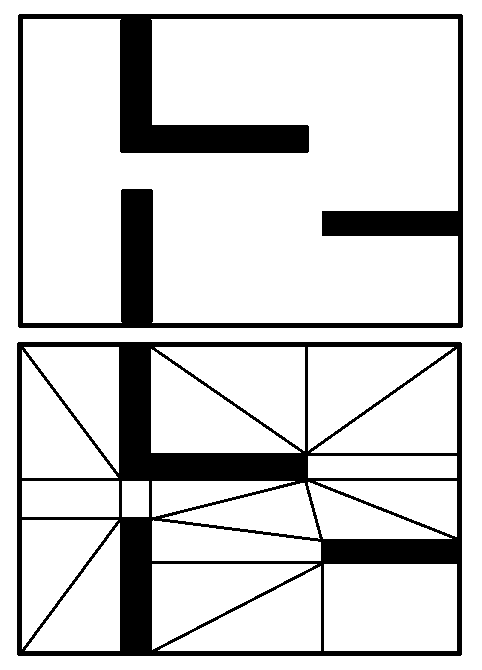
\includegraphics[scale=0.4]{graph_decomposition.png}
	\end{center}
	\caption{\label{fig:graph_decomp}
	     Arriba: Mapa de juego, los bloques negros son obstáculos.
	     Abajo: Partición del mapa del juego en polígonos convexos.}
\end{figure}

Adicionalmente, el número de agentes suele no ser
lo suficientemente grande para afectar significativamente
la complejidad del algoritmo. Casos extremos en los que
sea necesaria la utilización de un gran número de agentes,
se pueden solucionar con la agrupación de éstos bajo líderes
ficticios \cite{MF09}, de modo que por cada grupo se realice un solo
cálculo del camino. Naturalmente, mientras se agrupen los
individuos en conjuntos más grandes, la diversidad de
caminos se verá afectada negativamente.
\section{Trabajos Relacionados}

Un problema similar al aquí expuesto se da con \textit{Space-Time
 A$^*$} \cite{Sil06}, que plantea una variante de $A^*$ 
donde se tiene un grafo no dirigido en forma de cuadrícula,
 con función de costos común para todos los agentes y 
 constante entre cada par de nodos.

El objetivo principal de dicho trabajo es evitar el paso de
dos agentes por un mismo nodo en un instante de tiempo dado.
La variación planteada, incluye una extensión en el número
de dimensiones de $A^*$: se considera además de la posición
de los agentes, el tiempo transcurrido. Dicha variación tiene
un costo añadido en tiempo y memoria considerable debido a que
se incrementa el tamaño del espacio de búsqueda.

Aunque los algoritmos tienen objetivos diferentes, $A^*mbush$
presenta una clara ventaja sobre (\textit{Space-Time
 A$^*$}) en varios aspectos. 

En primer lugar, la solución propuesta en este artículo resuelve 
mediante un algoritmo de menor complejidad de cómputo
problemas más generales, debido a que permite grafos dirigidos
con costos variables. Asimismo se puede trabajar con agentes que
tengan grafos distintos entre sí.

Por otro lado, en el caso de tener agentes con distintas velocidades,
\textit{Space-Time A$^*$} genera un espacio de búsqueda en extremo
denso, cuando la velocidad relativa entre los e\-le\-men\-tos del juego es
alta. En cambio, $A^*mbush$ no se ve afectado por la diferencia de 
velocidades entre los agentes.

Asignando costos homogéneos para cada arco e incremento infinito
sobre nodos o arcos ocupados, el problema que resuelve $A^*mbush$
se reduce al problema planteado para \textit{Space-Time
A$^*$}.

\section{Experimentos}

Dada la naturaleza de los grafos de interés en el área de
videojuegos, la relación definida por los arcos es abstracta,
es decir, un agente no se encuentra realmente en un arco
entre un par de polígonos \cite{MF09}. Es por esto que en los
experimentos se considerará la variación de acumulación de
costos en nodos y no en arcos.

Para cada experimento se estudian tres algoritmos.
Una implementación base de $A*$ que sirve de referencia,
una implementación de generación de caminos simples pseudo-aleatorios
mediante búsqueda en profundidad, como me\-ca\-nis\-mo eficiente
que genere diversidad de caminos y por último, la variación
propuesta, $A^*mbush$.

Para el algoritmo $A^*$ se muestra el valor de emboscada
generado con dicho algoritmo ($\Phi_{A*}$). Para aleatorio
y $A^*mbush$, se muestra el incremento porcentual del costo
promedio de los caminos generados con cada método
($I_{Rand}$ e $I_{A^*mbush}$
respectivamente) en contraste con los costos
mínimos obtenidos por $A^*$ y el grado de emboscada ($\Phi$).

Serán considerados en los experimentos dos instancias de
mapas, la primera instancia (ver figura \ref{fig:g2}) cuenta con
60 polígonos y la segunda (ver figura \ref{fig:g1}) con 85. Todos los
polígonos son convexos para reducir el costo de la verificación
de pertenencia de un punto a un polígono \cite{Hai01}. Cada polígono
induce un nodo en el grafo ubicado en su centro geométrico \cite{MF09}.
Existen otras posibles convenciones para la discretización de los mapas
de juego, se utilizan estas convenciones dado que son las más
empleadas \cite{MF09}.
La función de costos es común para los agentes, se considera el costo
proporcional a la distancia euclidiana entre el centro de los
polígonos.

\begin{figure}[htb]
	\begin{center}
		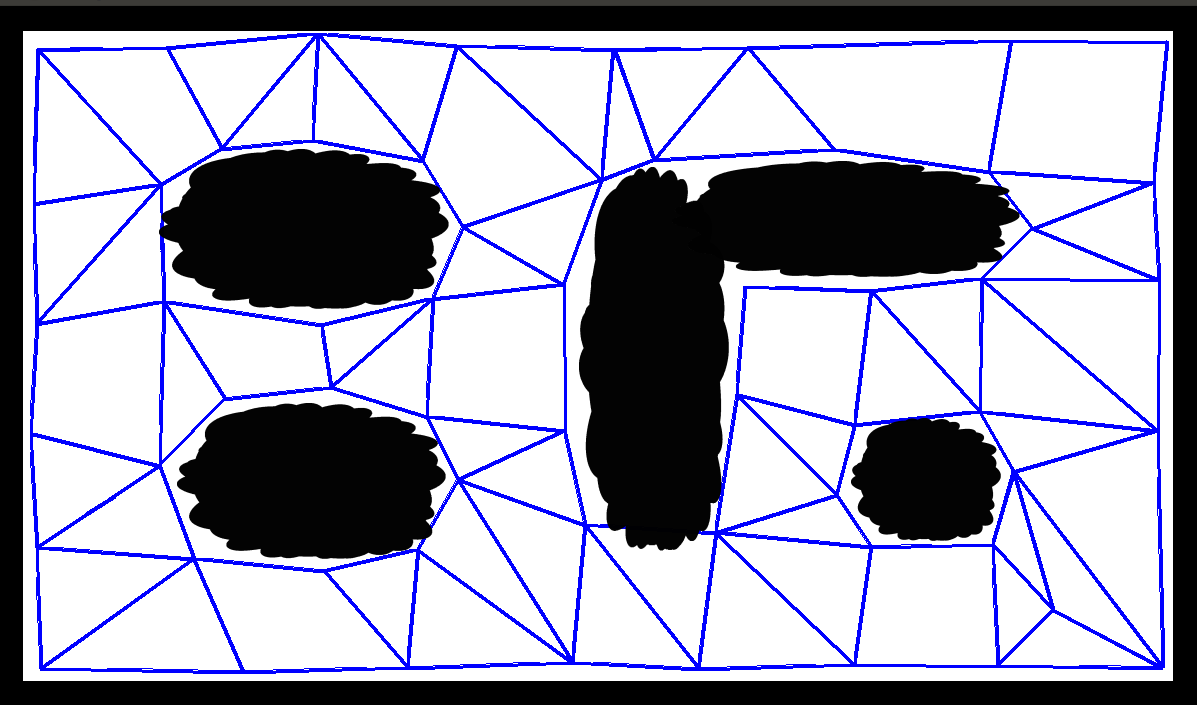
\includegraphics[scale=0.23]{g2.png}
	\end{center}
	\caption{\label{fig:g2}
	     Mapa 1 poligonalizado (60 polígonos).}
\end{figure}


\begin{figure}[htb]
	\begin{center}
		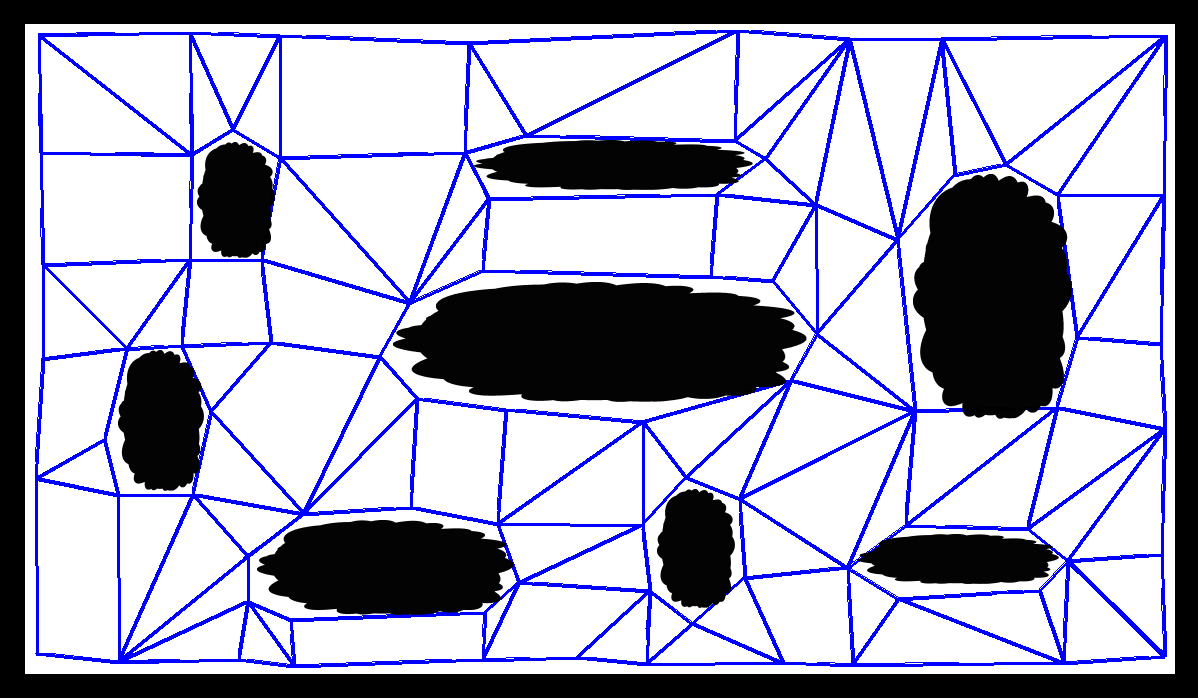
\includegraphics[scale=0.23]{g1.png}
	\end{center}
	\caption{\label{fig:g1}
	     Mapa 2 poligonalizado (85 polígonos).}
\end{figure}


En las secciones \ref{sec:3agentes} y \ref{sec:5agentes} se presentan
experimentos
 particulares con tres y cinco
agentes, respectivamente. Dado que los polígonos generados tienen a lo sumo
cuatro lados, es posible garantizar cobertura
máxima con cuatro agentes.

En los ejemplos correspondientes a agentes cercanos,
se disponen todos los agentes en el mismo polígono
inicial. En cambio, en los ejemplos con agentes alejados,
se coloca cada uno en polígonos diferentes distanciados.
Igualmente, se realizaron
experimentos variando el número de agentes, los resultados
correspondientes a dichos experimentos se describen en la sección \ref{sec:Globales}.
Los resultados señalados en negritas indican el máximo valor
de $\Phi$ encontrado.

\subsection{Experimentos con tres agentes}
\label{sec:3agentes}

\begin{table}[htb]
\begin{center}
\begin{tabular}{|l|r|r|r|r|r|r|}
\hline
\multicolumn{6}{|c|}{\textbf{Mapa 1 (60 nodos, 3 agentes)}}\\
\hline
$Ej$ & $\Phi_{A^*}$ & $I_{Rand}$ & $\Phi_{Rand}$
& $I_{A^*mbush}$ & $\Phi_{A^*mbush}$\\
\hline
\textit{a0} & 0.50 & 51.58 & \textbf{1.00} & 8.56 & \textbf{1.00} \\
\textit{a1} & \textbf{0.67} & 12.51 & 0.33 & 0.65 & \textbf{0.67} \\
\textit{a2} & \textbf{1.00} & 103.41 & 0.50 & 0.00 & \textbf{1.00} \\
\textit{a3} & 0.67 & 28.81 & 0.33 & 0.90 & \textbf{1.00} \\
\textit{a4} & \textbf{1.00} & 439.06 & 0.50 & 0.00 & \textbf{1.00} \\
\textit{a5} & \textbf{1.00} & 1.76 & \textbf{1.00} & 4.98 & \textbf{1.00} \\
\textit{a6} & \textbf{1.00} & 156.84 & \textbf{1.00} & 0.00 & \textbf{1.00} \\
\textit{a7} & \textbf{1.00} & 206.13 & 0.50 & 0.00 & \textbf{1.00} \\
\textit{a8} & \textbf{1.00} & 147.87 & \textbf{1.00} & 4.51 & \textbf{1.00} \\
\textit{a9} & \textbf{1.00} & 142.67 & 0.50 & 0.00 & \textbf{1.00} \\
\hline
\hline
\textit{c0} & 0.33 & 284.27 & 0.33 & 92.87 & \textbf{0.67} \\
\textit{c1} & 0.33 & 217.75 & 0.33 & 57.02 & \textbf{1.00} \\
\textit{c2} & 0.50 & 141.86 & 0.50 & 47.29 & \textbf{1.00} \\
\textit{c3} & 0.50 & 0.00 & 0.50 & 60.79 & \textbf{1.00} \\
\textit{c4} & 0.50 & 143.77 & 0.50 & 22.98 & \textbf{1.00} \\
\textit{c5} & 0.33 & 87.10 & 0.33 & 31.73 & \textbf{0.67} \\
\textit{c6} & 0.33 & 139.49 & 0.33 & 90.91 & \textbf{1.00} \\
\textit{c7} & 0.33 & 72.66 & 0.33 & 23.16 & \textbf{0.67} \\
\textit{c8} & 0.50 & 2.81 & 0.50 & 13.64 & \textbf{1.00} \\
\textit{c9} & 0.33 & 0.00 & 0.33 & 43.77 & \textbf{1.00} \\
\hline
\end{tabular}
\end{center}
	\caption{\label{tab:exp1}
	     Resultados de experimentos con tres agentes. Los casos
	     con $a_i$ se corresponden a ejemplos con agentes alejados
	     y los casos $c_i$ a agentes en el mismo polígono inicial.}
\end{table}

En la tablas \ref{tab:exp1} y \ref{tab:exp2} se presentan
los experimentos con tres agentes para el mapa uno y dos
respectivamente. En cada tabla, el primer bloque de experimentos
se corresponde a casos con agentes alejados, mientras que el
segundo a agentes ubicados inicialmente en el mismo polígono.

\begin{table}[htb]
\begin{center}
\begin{tabular}{|l|r|r|r|r|r|r|}
\hline
\multicolumn{6}{|c|}{\textbf{Mapa 2 (85 nodos, 3 agentes)}}\\
\hline
$Ej$ & $\Phi_{A^*}$ & $I_{Rand}$ & $\Phi_{Rand}$
& $I_{A^*mbush}$ & $\Phi_{A^*mbush}$\\
\hline
\textit{a0} & 0.67 & 242.81 & 0.33 & 4.95 & \textbf{1.00} \\
\textit{a1} & \textbf{0.50} & 62.04 & \textbf{0.50} & 0.72 & \textbf{0.50} \\
\textit{a2} & \textbf{1.00} & 254.91 & 0.50 & 0.00 & \textbf{1.00} \\
\textit{a3} & \textbf{1.00} & 891.31 & 0.50 & 5.66 & \textbf{1.00} \\
\textit{a4} & 0.50 & 252.42 & \textbf{1.00} & 11.15 & \textbf{1.00} \\
\textit{a5} & 0.50 & 43.63 & 0.50 & 10.08 & \textbf{1.00} \\
\textit{a6} & \textbf{1.00} & 498.94 & \textbf{1.00} & 0.00 & \textbf{1.00} \\
\textit{a7} & \textbf{1.00} & 261.09 & 0.50 & 10.42 & \textbf{1.00} \\
\textit{a8} & \textbf{0.67} & 39.64 & 0.33 & 0.00 & \textbf{0.67} \\
\textit{a9} & 0.50 & 386.92 & \textbf{1.00} & 9.37 & \textbf{1.00} \\
\hline
\hline
\textit{c0} & 0.50 & 344.86 & 0.50 & 114.95 & \textbf{1.00} \\
\textit{c1} & 0.33 & 22.20 & 0.33 & 7.40 & \textbf{0.67} \\
\textit{c2} & 0.50 & 24.70 & 0.50 & 58.64 & \textbf{1.00} \\
\textit{c3} & 0.50 & 64.63 & 0.50 & 8.48 & \textbf{1.00} \\
\textit{c4} & 0.33 & 303.53 & 0.33 & 17.12 & \textbf{0.67} \\
\textit{c5} & 0.50 & 354.85 & 0.50 & 90.76 & \textbf{1.00} \\
\textit{c6} & 0.33 & 956.07 & 0.33 & 83.64 & \textbf{0.67} \\
\textit{c7} & 0.33 & 141.46 & 0.33 & 23.36 & \textbf{0.67} \\
\textit{c8} & 0.50 & 1287.64 & 0.50 & 152.28 & \textbf{1.00} \\
\textit{c9} & 0.50 & 253.61 & 0.50 & 55.86 & \textbf{1.00} \\
\hline
\end{tabular}
\end{center}
	\caption{\label{tab:exp2}
	     Resultados de experimentos sobre el Mapa 2 con tres agentes. Los casos
	     con $a_i$ se corresponden a ejemplos con agentes alejados
	     y los casos $c_i$ a agentes en el mismo polígono inicial.}
\end{table}

En la tabla \ref{tab:exp1} se puede apreciar que $A^*mbush$
logra ser el mejor de las tres técnicas propuestas, mejorando
en la ma\-yo\-rí\-a de los casos la métrica de emboscada. Son de
particular interés los casos $a_2$ y todos los casos comprendidos
entre el $a_4$ y $a_9$, donde $A^*$ logra el valor máximo de
emboscada. En estos casos, $A^*mbush$ incrementa el costo promedio
de los caminos generados en a lo sumo $5\%$, por lo que se muestra
útil aún en casos donde la emboscada se da naturalmente.

Igualmente, casos como $a_0$, donde la versión pseudo-aleatoria
alcanza el mismo valor de $A^*mbush$, se aprecia un incremento
en el costo de los caminos considerable en contraste con la
variación propuesta. Teniendo para este caso
particular un incremento de $51.58\%$ para la versión aleatoria
y $8.56\%$ para $A^*mbush$.

En los casos donde los agentes parten de la misma posición inicial,
la mejora de $A^*mbush$ es considerable, logrando en su mayoría
maximizar el valor de la métrica de emboscada.

En la figura \ref{fig:ambush1} se puede apreciar
cómo tres agentes partiendo desde el mismo punto
toman caminos distintos generando una emboscada
al punto destino marcado con una cruz. Los caminos
mostrados se encuentran en bruto, es decir, se
muestran las uniones directas entre los centros
de los polígonos, generando movimientos bruscos.
Sin embargo, se pueden utilizar algoritmos de
suavizado de caminos \cite{MF09} para evitar cambios fuertes
en la orientación de los agentes.

\begin{figure}[htb]
	\begin{center}
		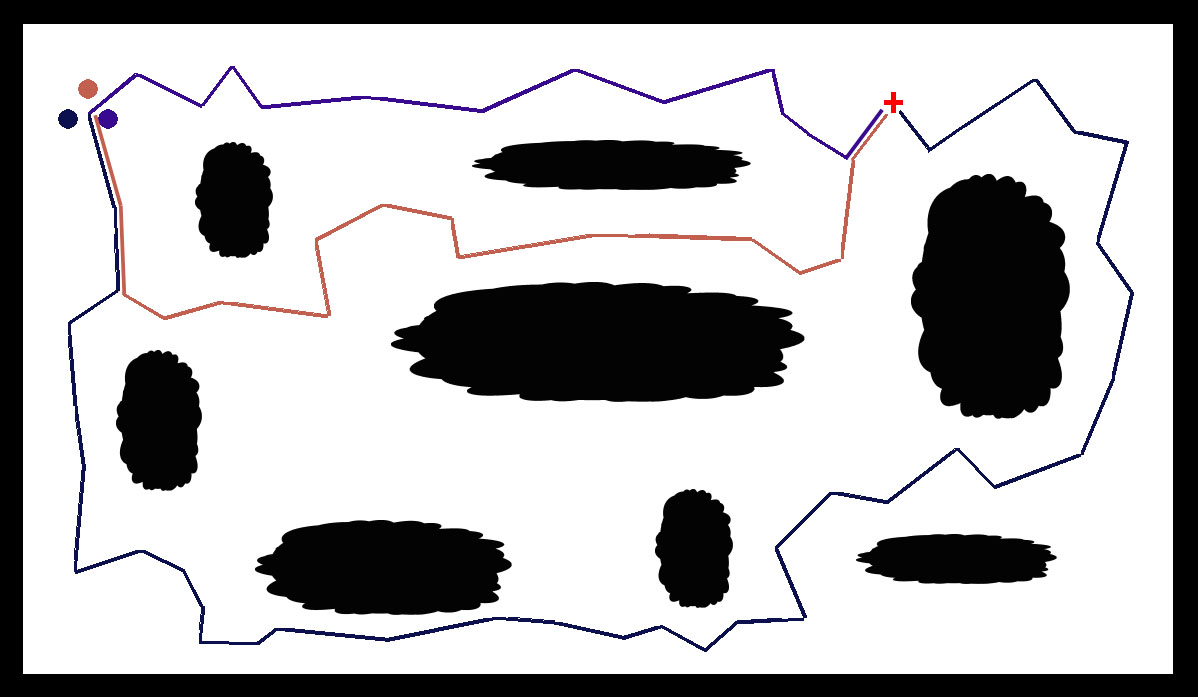
\includegraphics[scale=0.17]{ambush.jpg}
	\end{center}
	\caption{\label{fig:ambush1}
	     A*mbush en mapa 2 con tres agentes cercanos}
\end{figure}

\subsection{Experimentos con cinco agentes}
\label{sec:5agentes}

\begin{table}[htb]
\begin{center}
\begin{tabular}{|l|r|r|r|r|r|r|}
\hline
\multicolumn{6}{|c|}{\textbf{Mapa 1 (60 nodos, 5 agentes)}}\\
\hline
$Ej$ & $\Phi_{A^*}$ & $I_{Rand}$ & $\Phi_{Rand}$
& $I_{A^*mbush}$ & $\Phi_{A^*mbush}$\\
\hline
\textit{a0} & \textbf{1.00} & 129.89 & \textbf{1.00} & 5.14 & \textbf{1.00} \\
\textit{a1} & 0.67 & 7.51 & 0.33 & 7.02 & \textbf{1.00} \\
\textit{a2} & \textbf{1.00} & 128.00 & 0.50 & 8.57 & \textbf{1.00} \\
\textit{a3} & 0.67 & 18.55 & 0.33 & 9.98 & \textbf{1.00} \\
\textit{a4} & \textbf{1.00} & 289.28 & \textbf{1.00} & 0.00 & \textbf{1.00} \\
\textit{a5} & \textbf{1.00} & 1.06 & \textbf{1.00} & 21.72 & \textbf{1.00} \\
\textit{a6} & \textbf{1.00} & 119.92 & \textbf{1.00} & 30.52 & \textbf{1.00} \\
\textit{a7} & \textbf{1.00} & 181.23 & 0.50 & 6.90 & \textbf{1.00} \\
\textit{a8} & \textbf{1.00} & 147.59 & \textbf{1.00} & 11.64 & \textbf{1.00} \\
\textit{a9} & \textbf{1.00} & 142.83 & 0.50 & 9.33 & \textbf{1.00} \\
\textit{c0} & 0.33 & 284.27 & 0.33 & 112.58 & \textbf{0.67} \\
\hline
\hline
\textit{c1} & 0.33 & 217.75 & 0.33 & 37.11 & \textbf{1.00} \\
\textit{c2} & 0.50 & 141.86 & 0.50 & 111.15 & \textbf{1.00} \\
\textit{c3} & 0.50 & 0.00 & 0.50 & 104.96 & \textbf{1.00} \\
\textit{c4} & 0.50 & 143.77 & 0.50 & 49.69 & \textbf{1.00} \\
\textit{c5} & 0.33 & 87.10 & 0.33 & 20.66 & \textbf{0.67} \\
\textit{c6} & 0.33 & 139.49 & 0.33 & 54.55 & \textbf{1.00} \\
\textit{c7} & 0.33 & 72.66 & 0.33 & 48.81 & \textbf{1.00} \\
\textit{c8} & 0.50 & 2.81 & 0.50 & 36.49 & \textbf{1.00} \\
\textit{c9} & 0.33 & 0.00 & 0.33 & 92.86 & \textbf{1.00} \\
\hline
\end{tabular}
\end{center}
	\caption{\label{tab:exp3}
	     Resultados de experimentos sobbre el Mapa 1 con cinco agentes. Los casos
	     con $a_i$ se corresponden a ejemplos con agentes alejados
	     y los casos $c_i$ a agentes en el mismo polígono inicial.}
\end{table}

\begin{table}[htb]
\begin{center}
\begin{tabular}{|l|r|r|r|r|r|r|}
\hline
\multicolumn{6}{|c|}{\textbf{Mapa 2 (85 nodos, 5 agentes)}}\\
\hline
$Ej$ & $\Phi_{A^*}$ & $I_{Rand}$ & $\Phi_{Rand}$
& $I_{A^*mbush}$ & $\Phi_{A^*mbush}$\\
\hline
\textit{a0} & \textbf{1.00} & 223.75 & 0.33 & 24.19 & \textbf{1.00} \\
\textit{a1} & \textbf{1.00} & 122.20 & 0.50 & 6.76 & \textbf{1.00} \\
\textit{a2} & \textbf{1.00} & 284.70 & 0.50 & 9.59 & \textbf{1.00} \\
\textit{a3} & \textbf{1.00} & 562.86 & 0.50 & 10.97 & \textbf{1.00} \\
\textit{a4} & \textbf{1.00} & 185.77 & \textbf{1.00} & 1.08 & \textbf{1.00} \\
\textit{a5} & 0.50 & 26.88 & 0.50 & 19.96 & \textbf{1.00} \\
\textit{a6} & \textbf{1.00} & 386.65 & \textbf{1.00} & 4.84 & \textbf{1.00} \\
\textit{a7} & \textbf{1.00} & 216.45 & 0.50 & 28.72 & \textbf{1.00} \\
\textit{a8} & 0.50 & 37.85 & 0.25 & 25.38 & \textbf{1.00} \\
\textit{a9} & 0.50 & 310.39 & \textbf{1.00} & 5.62 & \textbf{1.00} \\
\hline
\hline
\textit{c0} & 0.50 & 344.86 & 0.50 & 68.97 & \textbf{1.00} \\
\textit{c1} & 0.33 & 22.20 & 0.33 & 83.28 & \textbf{1.00} \\
\textit{c2} & 0.50 & 24.70 & 0.50 & 44.61 & \textbf{1.00} \\
\textit{c3} & 0.50 & 64.63 & 0.50 & 6.49 & \textbf{1.00} \\
\textit{c4} & 0.25 & 303.53 & 0.25 & 83.31 & \textbf{0.75} \\
\textit{c5} & \textbf{1.00} & 332.13 & \textbf{1.00} & 55.54 & \textbf{1.00} \\
\textit{c6} & 0.33 & 956.07 & 0.33 & 135.02 & \textbf{1.00} \\
\textit{c7} & 0.33 & 141.46 & 0.33 & 43.96 & \textbf{1.00} \\
\textit{c8} & 0.50 & 1287.64 & 0.50 & 91.37 & \textbf{1.00} \\
\textit{c9} & 0.50 & 253.61 & 0.50 & 34.54 & \textbf{1.00} \\
\hline
\end{tabular}
\end{center}
	\caption{\label{tab:exp4}
	     Resultados de experimentos sobre el Mapa 2 con cinco agentes. Los casos
	     con $a_i$ se corresponden a ejemplos con agentes alejados
	     y los casos $c_i$ a agentes en el mismo polígono inicial.}
\end{table}

En las tabla \ref{tab:exp3} y \ref{tab:exp4} se 
aprecian experimentos análogos a los expuestos en
las tablas \ref{tab:exp1} y \ref{tab:exp2}, pero
con un total de cinco agentes.

A diferencia de los experimentos con tres agentes,
en los experimentos con cinco agentes, se logró
mejorar en todos los casos posibles la calidad de
la emboscada. Es importante destacar que, si
bien el valor de incremento del costo de los caminos
tiende a aumentar con el número de agentes, $A^*mbush$
logra mejorar cuantitativamente el comportamiento de estos.

En la figura \ref{fig:ambush2} se puede apreciar una gran
diversidad de caminos seleccionados. Nótese que adicionalmente
a haber generado una emboscada, los agentes se distribuyeron a
lo largo del mapa.

\begin{figure}[htb]
	\begin{center}
		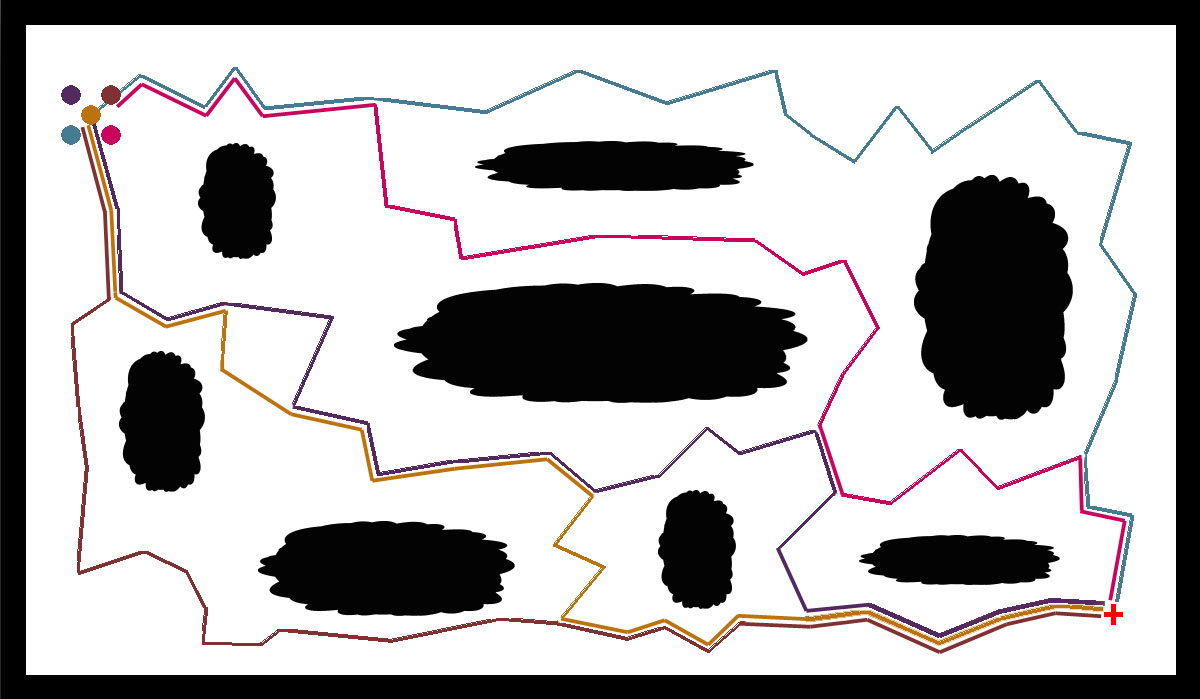
\includegraphics[scale=0.17]{ambush2.jpg}
	\end{center}
	\caption{\label{fig:ambush2}
	     Ambush en mapa 1 con cinco agentes cercanos}
\end{figure}

\subsection{Experimentos Globales}
\label{sec:Globales}

En las tablas \ref{tab:g1} y \ref{tab:g2} se muestran
resultados globales de cada mapa variando el número de
agentes. Para cada caso, se generaron 1000 casos aleatorios
de distribución de los agentes en los polígonos. Cada una de
las distribuciones aleatorias se compara colocando como objetivo
cada uno de los polígonos del grafo. Finalmente se promedian
los resultados obtenidos para cada métrica.

No se realizó la exploración
completa en el espacio de posibilidades dado su rápido crecimiento.
De ser necesario disponer $k$ agentes en un grafo con $|V|$ nodos,
el número total de combinaciones es de $|V|^{k+1}$, cada una de esas
combinaciones debe ejecutar los mecanismos propuestos para cada
agente, por lo que la complejidad total sería
$\bigO( (|V|log|V| + |E|)\cdot k \cdot |V|^{k+1} )$.

\begin{table}[htb]
\begin{center}
\begin{tabular}{|l|r|r|r|r|r|r|}
\hline
\multicolumn{6}{|c|}{\textbf{Mapa 1 (60 nodos, 3-20 agentes)}}\\
\hline
$\#$ & $\Phi_{A^*}$ & $I_{Rand}$ & $\Phi_{Rand}$
& $I_{A^*mbush}$ & $\Phi_{A^*mbush}$\\
\hline
 3 & 0.78 & 406.85 & 0.78 & 11.81 & \textbf{0.95}\\
 4 & 0.84 & 403.67 & 0.84 & 15.53 & \textbf{0.99}\\
 5 & 0.86 & 402.89 & 0.87 & 17.88 & \textbf{0.99}\\
 6 & 0.90 & 405.26 & 0.89 & 19.33 & \textbf{1.00}\\
 7 & 0.91 & 406.06 & 0.91 & 20.63 & \textbf{1.00}\\
 8 & 0.93 & 405.29 & 0.92 & 20.81 & \textbf{1.00}\\
 9 & 0.94 & 403.61 & 0.93 & 21.25 & \textbf{1.00}\\
10 & 0.95 & 404.69 & 0.94 & 21.67 & \textbf{1.00}\\
11 & 0.96 & 405.28 & 0.94 & 21.94 & \textbf{1.00}\\
12 & 0.97 & 405.45 & 0.95 & 21.92 & \textbf{1.00}\\
13 & 0.97 & 405.87 & 0.95 & 21.97 & \textbf{1.00}\\
14 & 0.98 & 405.12 & 0.95 & 22.19 & \textbf{1.00}\\
15 & 0.98 & 403.69 & 0.96 & 22.14 & \textbf{1.00}\\
16 & 0.98 & 403.07 & 0.96 & 21.95 & \textbf{1.00}\\
17 & 0.99 & 405.29 & 0.96 & 22.01 & \textbf{1.00}\\
18 & 0.99 & 405.13 & 0.96 & 21.93 & \textbf{1.00}\\
19 & 0.99 & 403.78 & 0.96 & 21.82 & \textbf{1.00}\\
20 & 0.99 & 403.50 & 0.97 & 21.75 & \textbf{1.00}\\
\hline
\end{tabular}
\end{center}
	\caption{\label{tab:g2}
	     Resultados de experimentos con número variable de agentes
	     para el Mapa 1.}
\end{table}
\begin{table}[htb]
\begin{center}
\begin{tabular}{|l|r|r|r|r|r|r|}
\hline
\multicolumn{6}{|c|}{\textbf{Mapa 2 (85 nodos, 3-20 agentes)}}\\
\hline
$\#$ & $\Phi_{A^*}$ & $I_{Rand}$ & $\Phi_{Rand}$
& $I_{A^*mbush}$ & $\Phi_{A^*mbush}$\\
\hline
 3 & 0.77 & 407.06 & 0.78 & 12.08 & \textbf{0.95}\\
 4 & 0.83 & 409.85 & 0.84 & 15.64 & \textbf{0.99}\\
 5 & 0.87 & 403.54 & 0.87 & 17.67 & \textbf{0.99}\\
 6 & 0.90 & 403.63 & 0.89 & 19.32 & \textbf{1.00}\\
 7 & 0.92 & 404.63 & 0.91 & 19.86 & \textbf{1.00}\\
 8 & 0.94 & 403.69 & 0.92 & 20.66 & \textbf{1.00}\\
 9 & 0.94 & 404.42 & 0.93 & 21.56 & \textbf{1.00}\\
10 & 0.95 & 403.30 & 0.94 & 21.54 & \textbf{1.00}\\
11 & 0.96 & 402.53 & 0.94 & 21.95 & \textbf{1.00}\\
12 & 0.97 & 404.34 & 0.95 & 21.85 & \textbf{1.00}\\
13 & 0.97 & 405.51 & 0.95 & 21.97 & \textbf{1.00}\\
14 & 0.98 & 403.64 & 0.95 & 22.09 & \textbf{1.00}\\
15 & 0.98 & 404.98 & 0.96 & 22.19 & \textbf{1.00}\\
16 & 0.98 & 403.45 & 0.96 & 21.94 & \textbf{1.00}\\
17 & 0.98 & 404.12 & 0.96 & 21.95 & \textbf{1.00}\\
18 & 0.99 & 404.21 & 0.96 & 21.94 & \textbf{1.00}\\
19 & 0.99 & 404.70 & 0.96 & 21.98 & \textbf{1.00}\\
20 & 0.99 & 404.67 & 0.96 & 21.90 & \textbf{1.00}\\
\hline
\end{tabular}
\end{center}
	\caption{\label{tab:g1}
	     Resultados de experimentos con número variable de agentes
	     para el Mapa 2.}
\end{table}

Es importante notar de las tablas \ref{tab:g1} y
\ref{tab:g2} como al incrementar el número de agentes,
el grado de emboscada de las tres estrategias planteadas
aumenta. Sin embargo, $A^*bmush$ logra situarse
en todos los casos por encima de las demás estrategias.
Logrando a partir de seis agentes para ambos grafos
propuestos alcanzar en cada caso el valor óptimo de
emboscada, en paralelo con un bajo incremento porcentual
en el costo de los caminos de los agentes.

\section{Análisis de los Resultados}

Se puede observar que $A^*mbush$ genera de manera
efectiva incrementar el valor de emboscada, comparado
con la estrategia tradicional de búsqueda de caminos
$A^*$. Si bien en ciertos casos no logra una mejora
de esta métrica, es notable en la práctica la diversidad
de estos caminos. Nótese que la métrica de evaluación
sólo considera el segmento final de los caminos obtenidos.
Por otro lado, a diferencia de métodos de generación
de caminos diversos como el pseudo-aleatorio, el incremento
en el costo de los caminos obtenidos se mantiene en rangos
razonables.

En los experimentos desarrollados, $A^*mbush$ no varía
significativamente con respecto al número de polígonos.
En cambio, se puede apreciar cómo la posición inicial de
los agentes, puede afectar el desenvolvimiento del algoritmo.
A medida que los agentes se encuentren más dispersos en el
mapa, la mejora de $A^*mbush$ con respecto a $A^*$ no
es significativa, debido a que es menos probable que
existan nodos o arcos comunes en los caminos de los agentes.

En cambio, cuando los agentes se encuentran concentrados
en regiones pequeñas del mapa, $A^*mbush$ genera una mejora
significativa en el valor de $\Phi$.

Es importante destacar que el incremento en el costo de
los caminos obtenidos por $A^*mbush$ no crece indefinidamente,
como se puede ver en los experimentos globales,
dado que cuando los agentes abarcan todos los arcos del grafo,
los incrementos por nodo o por arco tienden a ser homogéneos.

Una gran ventaja de $A^*mbush$ es que, como favorece a una
rápida dispersión de los agentes a lo largo del mapa, si
el objetivo a alcanzar se encuentra en movimiento, se genera
un mayor número de posiciones de emboscada.

En la figura \ref{fig:contraste} se puede contrastar el resultado
de los tres mecanismos planteados para un caso particular.
Nótese que en el caso de $A^*$ los tres agentes llegaron al destino
desde el mismo sector utilizando sus caminos más cortos. Para el
aleatorio, el comportamiento fue similar al caso de $A^*$, sin
embargo tomaron todos un camino significativamente más largo.
En cambio, $A^*mbush$ logró que uno de los agentes tomara
un camino distinto, logrando alcanzar al objetivo desde los
dos flancos posibles.

\begin{figure}[htb]
	\begin{center}
		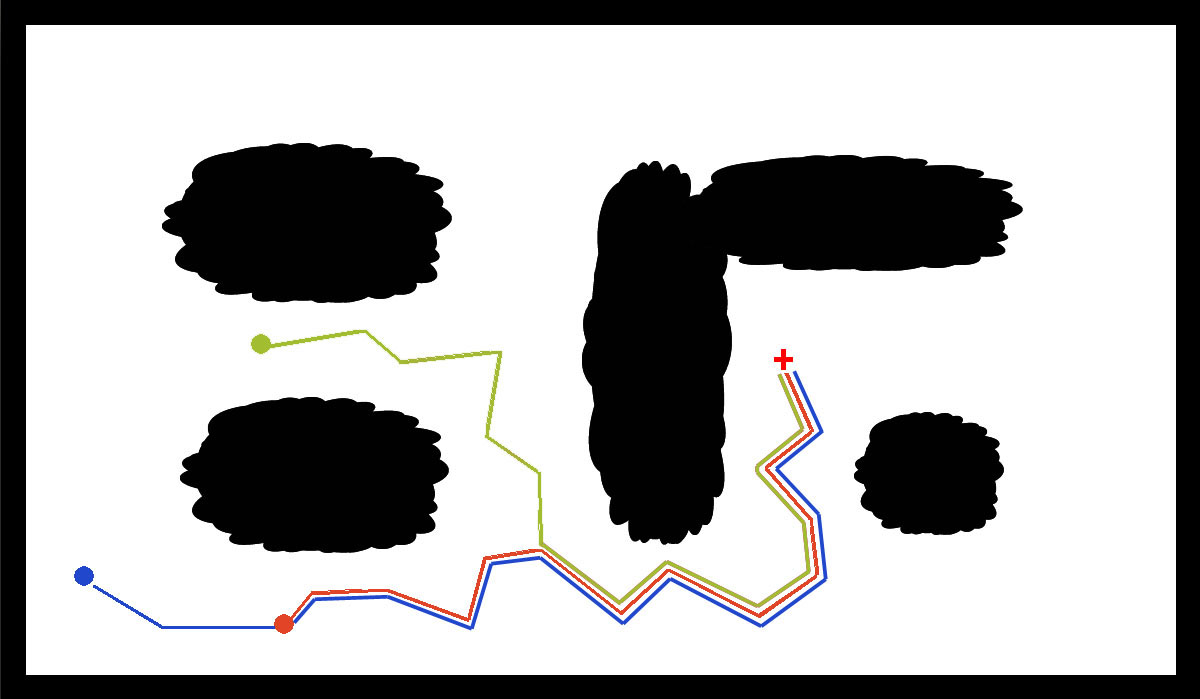
\includegraphics[scale=0.17]{astar_contrast.jpg}\\
		\vspace{0.1cm}
		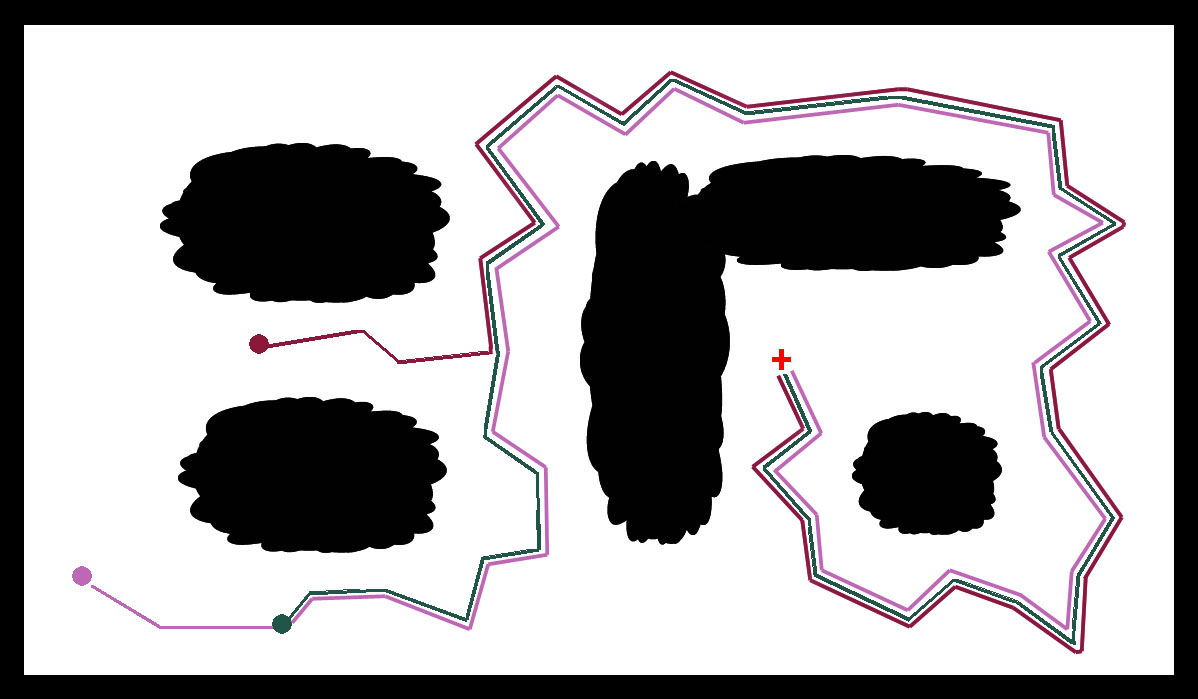
\includegraphics[scale=0.17]{dfs_contrast.jpg}\\
		\vspace{0.1cm}
		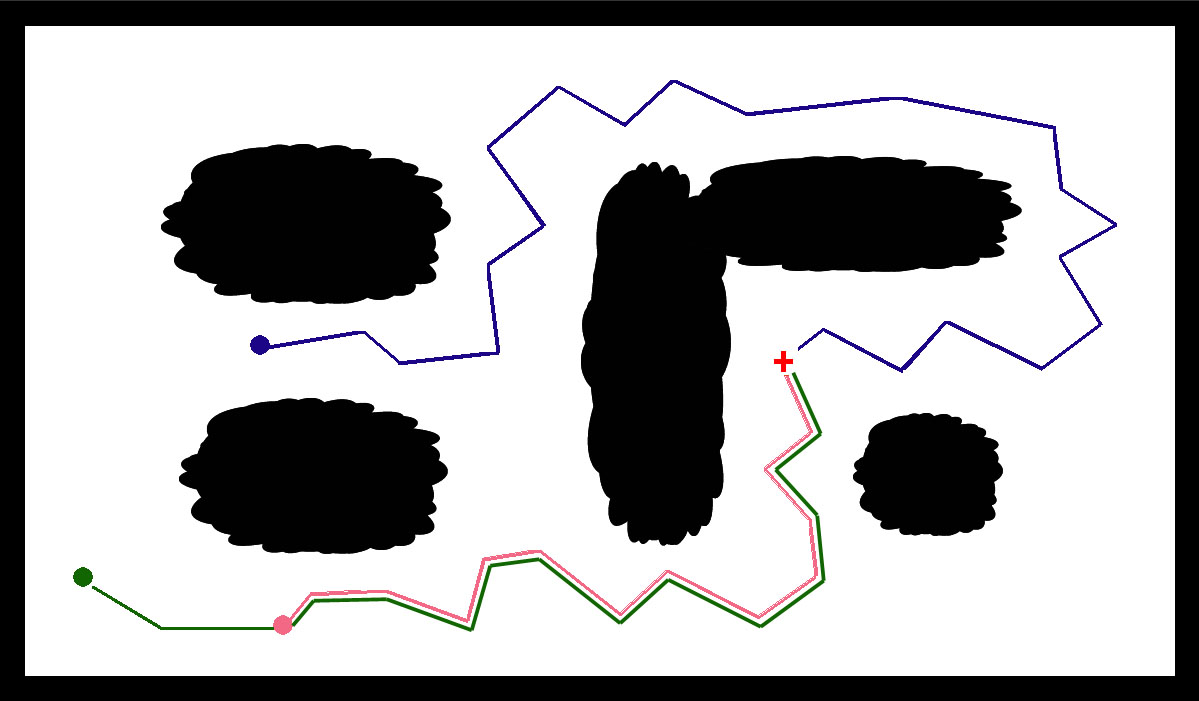
\includegraphics[scale=0.17]{ambush_contrast.jpg}\\
	\end{center}
	\caption{\label{fig:contraste}
	     Caminos generados por tres agentes utilizando respectivamente
	     $A^*$, pseudo-aleatorio y $A^*mbush$ (de arriba hacia abajo).}
\end{figure}

\section{Conclusiones}

Con un aumento en el costo de cómputo poco significativo, 
$A^*mbush$ genera una evidente mejora en la conducta de emboscada. 
También diversifica exitosamente los caminos que seleccionan
los agentes.

Como se puede apreciar en los resultados, en el peor de los casos
el algoritmo propuesto no cambia el grado de emboscada, es decir,
aún en la situación menos favorable, $A^*mbush$ nunca genera un peor 
resultado que el obtenido con $A^*$.

Al diversificarse los caminos, los agentes naturalmente se distribuyen con
mayor uniformidad en el mapa. Esto puede ser ventajoso en el caso de un 
cambio de estado a una nueva conducta, en el que sea conveniente que los
agentes no estén conglomerados en un punto. Por ejemplo, si se cambia
de conducta de persecución a huída, $A^*mbush$ no sólo permite un
comportamiento de emboscada, sino que mantiene a los agentes más 
alejados los unos de los otros, dejándolos en una posición más adecuada
para escapar.

$A^*mbush$ genera comportamientos de emboscada inteligentes
para situaciones en las que múltiples agentes necesitan
alcanzar un objetivo común. En contraste con estrategias preestablecidas,
regularmente implementadas para situaciones específicas de cada juego,
que derivan en situaciones repetitivas, $A^*mbush$ logra fomentar
situaciones va\-ria\-das de emboscada dentro del comportamiento
táctico grupal de los agentes.

\subsection{Aplicación a un Videojuego}

$A^*mbush$ ha sido implementado en el juego FatBoy para la
materia ``Tópicos en Inteligencia Artificial: Juegos'' de la
Universidad Simón Bolívar. El juego puede ser consultado en
http://www.gia.usb.ve/wikis/iajuegos/Kelwin\%20Fernández. 

En http://www.gia.usb.ve/$\sim$kelwin/research/sctc2012/
pueden encontrarse casos de interés adicionales.

\section{Otras Aplicaciones}

La diversificación de caminos generada por $A^*mbush$ no se limita a su
aplicación al área de videojuegos.

En el caso de las redes, $A^*mbush$ puede utilizarse para generar menor 
congestión en el envío de paquetes, generando una mayor diversidad
en el uso de la red \cite{TMSV03}. Los enrutadores pueden sincronizar 
cada cierto tiempo su información con los demás, para poder tomar 
en cuenta la cantidad de paquetes en cada punto. De esta forma es
posible generar un uso más uniforme de los canales de una red.

$A^*mbush$ también consigue una natural aplicación en la planificación
del tráfico de vehículos. Utilizando la segunda versión propuesta
(incremento de costos en arcos), se puede generar una planificación
favorezca el uso de rutas más largas y poco transitadas, para aligerar el embotellamiento general.

En el desarrollo de algoritmos heurísticos de optimización, tales
como GRASP, Colonia de Hormigas, entre otros \cite{GP10}, es posible generar
una mayor diversificación en el espacio de búsqueda utilizando
variaciones de $A^*mbush$ adaptadas al contexto del problema.

Finalmente, la variación expuesta en el presente trabajo no se
limita al algoritmo particular de $A^*$. La idea
central de $A^*mbush$ es el cómputo de una nueva función de
costos que penalice los sectores del grafo más utilizados, por
lo que el mismo enfoque puede ser implementado en otros algoritmos
de cómputo de caminos en grafos con costos, tales como $IDA^*$,
\textit{Fringe Search}, \textit{Branch and Bound}, entre otros.

\section{Trabajos Futuros}

Debido a la naturaleza del algoritmo, es posible que un agente
que se encuentra cerca del objetivo, deba desviarse dado que
otros agentes han tomado arcos de interés para éste previamente.
Se explorarán variaciones que incluyan prioridades a los agentes
para reducir el incremento porcentual del costo de los caminos
obtenidos. También se explorará la posibilidad de incorporar
selectivamente el algoritmo de A$^*$mbush, siguiendo criterios
tales como la cercanía del agente al objetivo, con el fin de
minimizar el incremento promedio de los caminos.

% ESTO NOS HARIA CAER EN LA DISCUSION DE SPACE-TIME
%Adicionalmente, se propondrán alternativas donde el incremento
%en el costo de un arco o nodo se considere sólo en el momento
%en que dos o más agentes deseen pasar por el mismo punto en
%intervalos de tiempos solapados.

Igualmente, se trabajará incluyendo capacidad máxima a los nodos
y arcos. Nótese que esta variación responde al problema propuesto
en \cite{Sil06} cuando cada arco tiene capacidad unitaria.

Adicionalmente, se implementará una heurística que le permita
a los agentes sólo utilizar $A^*mbush$ cuando estén dentro de 
cierto radio cercano al objetivo. Logrando de esta manera reducir el 
costo, tanto de cálculo como el de los caminos. Esta heurística también
puede adaptarse para generar distintas dificultades de juego.

\bibliographystyle{eg-alpha}

\bibliography{egbibsample}

\end{document}
